%; whizzy paragraph -pdf xpdf -latex ./whizzypdfptex.sh
%; whizzy-paragraph "^\\\\begin{frame}\\|\\\\emtext"
% latex beamer presentation.
% platex, latex-beamer でコンパイルすることを想定。 

%     Tokyo Debian Meeting resources
%     Copyright (C) 2012 Junichi Uekawa

%     This program is free software; you can redistribute it and/or modify
%     it under the terms of the GNU General Public License as published by
%     the Free Software Foundation; either version 2 of the License, or
%     (at your option) any later version.

%     This program is distributed in the hope that it will be useful,
%     but WITHOUT ANY WARRANTY; without even the implied warreanty of
%     MERCHANTABILITY or FITNESS FOR A PARTICULAR PURPOSE.  See the
%     GNU General Public License for more details.

%     You should have received a copy of the GNU General Public License
%     along with this program; if not, write to the Free Software
%     Foundation, Inc., 51 Franklin St, Fifth Floor, Boston, MA  02110-1301 USA

\documentclass[cjk,dvipdfmx,12pt]{beamer}
\usetheme{Tokyo}
\usepackage{monthlypresentation}

%  preview (shell-command (concat "evince " (replace-regexp-in-string "tex$" "pdf"(buffer-file-name)) "&")) 
%  presentation (shell-command (concat "xpdf -fullscreen " (replace-regexp-in-string "tex$" "pdf"(buffer-file-name)) "&"))
%  presentation (shell-command (concat "evince " (replace-regexp-in-string "tex$" "pdf"(buffer-file-name)) "&"))

%http://www.naney.org/diki/dk/hyperref.html
%日本語EUC系環境の時
\AtBeginDvi{\special{pdf:tounicode EUC-UCS2}}
%シフトJIS系環境の時
%\AtBeginDvi{\special{pdf:tounicode 90ms-RKSJ-UCS2}}

\newenvironment{commandlinesmall}%
{\VerbatimEnvironment
  \begin{Sbox}\begin{minipage}{1.0\hsize}\begin{fontsize}{8}{8} \begin{BVerbatim}}%
{\end{BVerbatim}\end{fontsize}\end{minipage}\end{Sbox}
  \setlength{\fboxsep}{8pt}
% start on a new paragraph

\vspace{6pt}% skip before
\fcolorbox{dancerdarkblue}{dancerlightblue}{\TheSbox}

\vspace{6pt}% skip after
}
%end of commandlinesmall

\title{東京エリアDebian勉強会}
\subtitle{第102回 2013年7月度}
\author{上川純一}
\date{2013年7月20日}
\logo{
\includegraphics[width=8cm]{image200607/openlogo-light.eps}}

\begin{document}

\begin{frame}
\titlepage{}
\end{frame}

\begin{frame}{設営準備にご協力ください。}
会場設営よろしくおねがいします。
\end{frame}

\begin{frame}{Agenda}
\begin{minipage}[t]{0.45\hsize}
  \begin{itemize}
  \item 注意事項
	\begin{itemize}
	 \item 飲食禁止
	\end{itemize}
   \item 最近あったDebian関連のイベント報告
	\begin{itemize}
        \item 第100回 東京エリアDebian勉強会
        \item 2013 大統一Debian勉強会
	\end{itemize}
 \end{itemize}
\end{minipage} 
\begin{minipage}[t]{0.45\hsize}
 \begin{itemize}
  \item Debian Trivia Quiz
  \item 事前課題紹介
 \end{itemize}
\end{minipage}
\end{frame}

\section{イベント報告}
\emtext{イベント報告}

\begin{frame}{第100回 東京エリアDebian勉強会}
  
\end{frame}

\begin{frame}{大統一Debian勉強会 2013}
\end{frame}

\section{DWN quiz}
\emtext{DWN quiz}
\begin{frame}{Debian 常識クイズ}

  Debian の常識、もちろん知ってますよね?
知らないなんて恥ずかしくて、知らないとは言えないあんなことやこんなこと、
みんなで確認してみましょう。

今回の出題範囲は\url{debian-devel-announce@lists.debian.org},
\url{debian-devel@lists.debian.org} に投稿された
内容とDebian Project Newsなどからです。

\end{frame}

\subsection{問題}
%; whizzy-master ../debianmeetingresume201211.tex
% 以上の設定をしているため、このファイルで M-x whizzytex すると、whizzytexが利用できます。
%

\santaku
{Stefano Zacchiroli さんが新しく作成したサービスは?}
{chiebukuro.debian.net}
{2ch.debian.net}
{sources.debian.net}
{C}
{Stefano Zacchiroli さんが、Debian パッケージで提供されているソースコードすべてを閲覧・検索出来るsources.debian.netを作った}

\santaku
{新しく FTP master チームに入った人は?}
{Gergely Nagy} % 2012 DPL立候補者 % dh-exec 開発者
{Kouhei Maeda}
{Joerg Jaspert}
{A}
{Paul Tagliamonte,Scott Kitterman,Luke Faraone, Gergely Nagy が加入}

\santaku
{Debian GNU/Hurd がリリースされましたが、バージョンはいくつでしょう。}
{2013}
{3.141592}
{7.0}
{A}
{}



\section{事前課題}
\emtext{事前課題}

%今回の事前課題は以下のような内容でした。
%\begin{enumerate}
%\item お使いのマシンにARMはありますか?もしあるのでしたら、どのように使っ
%ているか教えてください。
%\item  Debian のARM に期待していること、お願いしたいことがあれば教えてくだ
%さい。
%\end{enumerate}
{\footnotesize
 
\begin{prework}{ koedoyoshida }

\begin{enumerate}
\item お使いのマシンにARMはありますか?もしあるのでしたら、どのように使っ
ているか教えてください。\\
Raspberry Piを使ってます。
とりあえずリモートアクセス用がメインですが、
I2Cとかを使って外部IOをやってみたいと思っています。
\item  Debian のARM に期待していること、お願いしたいことがあれば教えてくだ
さい。\\
省電力な環境を生かしてReadOnlyboot(でも定期的にセキュリティupdateはし
たい)で放置できる環境とかが作れるとよいですね。
\end{enumerate}

\end{prework}

\begin{prework}{ 吉野 }
\begin{enumerate}
\item  地図マシンです
\item なし 
\end{enumerate}
\end{prework}

\begin{prework}{ dictoss}
\begin{enumerate}
\item  CuBoxを持っている。eSATA端子があるのでファイルサーバのバックアップ
をするマシンとして使おうとしたが、USBポートから電源供給量が不足のため、
HDDが動かず使えていない。そのため単なるarmelバイナリのお試しマシンになっ
ている。

\item  新Nexus7でDebianが動いてほしい。
\end{enumerate}
\end{prework}

\begin{prework}{ mtoshi.g }
\begin{enumerate}
\item  お使いのマシンにARMはありますか?\\
ないっす

\item  Debian のARM に期待していること、お願いしたいことがあれば教えてくだ
さい。\\
今のところないっす
\end{enumerate}
\end{prework}

\begin{prework}{ 野島 貴英 }
\begin{enumerate}
\item  昔売っていたB\&NのNookColorをARM機材実験ボードとして未だに使ってます。
この電子書籍端末は2012/4の東京エリアdebian勉強会,2012/6の大統一debian
勉強会で喋ったとおり、特定ブートフォーマットのSDカードを用意してSDカー
ドスロットへ入れちゃうと、うっかりそのままブートしちゃうという隠れ(?)
機能が大変便利です。おまけに連続8回起動失敗するとリカバリーが始まると
いう非文鎮化機能まで搭載しています。そのままでもpdfリーダ、ポータブル
mp4ビデオ/mp3鑑賞機材として、また、debian ARMのnativeブートの可能性を
秘めたhack機材としても楽しくお使いいただけます。
\item  NookColor用のdebianネイティブブートが可能なイメージ(というかインス
  トーラ)が欲しいといってみるテスト。
\end{enumerate}
\end{prework}

\begin{prework}{ 岩松 信洋 }
\begin{enumerate}
\item  お使いのマシンにARMはありますか?もしあるのでしたら、どのように使っ
ているか教えてください。\\
たくさんある。開発用とかビルドマシンとして使っています。
Raspberry Pi は家のゲートウェイマシンとして動いています。
\item  Debian のARM に期待していること、お願いしたいことがあれば教えてくだ
さい。\\
マルチメディア系が弱いので整備して欲しい。
\end{enumerate}

\end{prework}

\begin{prework}{ 上川純一 }
なし
\end{prework}

\begin{prework}{ まえだこうへい }
\begin{enumerate}
\item  Armadillo Jで自宅内のDHCPサーバとして使っています(not Debian)。
OpenBlockS AX3を、昨年夏ごろにカッとなって作ったioriというツール(最近
話題のdockerみたいなの)の開発環境として使っています。
\item  今は特にないですが、今後ARMサーバの製品版が出てきた時にd-iでインス
トールできることでしょうか。
\end{enumerate}
\end{prework}

}

\section{armmp}
\emtext{armmp}

\section{月刊Debhelper}
\emtext{月刊Debhelper}
\begin{frame}{今月のコマンド}
\begin{center}
\Huge
 dh\_strip
\end{center}
\end{frame}

\begin{frame}{dh\_stripの機能}

\begin{itemize}
\item 実行バイナリ、共有ライブラリ、静的ライブラリから、デバッグシンボルを取り除く。
\item 取り除いたデバッグシンボルをデバッガが見つけれるようにして、*-dbgパッケージが作りやすいようにビルドディレクトリ以下に配置する
\end{itemize}

\end{frame}

\begin{frame}{どうやって*-dbgパッケージを作る?}

 そんなあなたに、\\
\begin{center}
\LARGE
2012年 大統一Debian勉強会\\
「debug.debian.net」の\\
プレゼン資料がおすすめ!
\end{center}
\begin{center}
\url{http://gum.debian.or.jp/2012/}
\end{center}

 とりあえず、すでに発表済みなので、ここでは省略。

\end{frame}

\begin{frame}{dh\_stripのコマンドラインオプション(その1)}

\begin{itemize}
\item man debhelperに記載されているdebhelper共通オプション\\
 他の月刊debhelperの発表でなされているとおりなので、ここでは割愛。
\item -Xitem,--exclude=item \\
  itemという名前を持つファイル名に対しては処理を行いません。複数指定したければ、
``dh\_strip -Xfoo1 -Xfoo2''と複数ならべて指定ができます。
\item --dbg-package=package \\
*-dbgパッケージを作る際に、デバッグシンボルを格納するパッケージ名を指定する為に利用します。debhelperのCOMPATIBILITY LEVELによって振る舞いが変わります。(後述)
\end{itemize}

\end{frame}

\begin{frame}{dh\_stripのコマンドラインオプション(その2)}
\begin{itemize}
\item -k \\
デバッグシンボルをバイナリパッケージに含めてしまいます。つまり、バイナリがインストールされると同時に、対応したデバッグシンボルも/usr/lib/debug/以下にインストールされるようなパッケージを作成するときに使います。なお、--dbg-packageも指定されると、--dbg-packageの方の動作が優先されます。
\end{itemize}

\end{frame}

\begin{frame}{dh\_stripのCOMPATIBILITY LEVELの動作の違い(その1)}

以下は--dbg-package指定時のdh\_stripの振る舞いの違い。

\begin{itemize}
\item 4以下\\
 ``dh\_strip --dbg-package=xxxx --dbg-package=yyyy''のように--dbg-package
を複数指定する事が出来ます。ここで、こちらで指定した名前(xxxxや、yyyy)に合致する
パッケージを処理する際、''パッケージ名-dbg''というパッケージ名を*-dbgパッケージ
のパッケージ名として自動的に利用します。また、このCOMPATIBILITY LEVELの場合、
ソースパッケージに含まれるdebian/controlには、これら*-dbgパッケージの為の
記述を必要とはしていません。
\end{itemize}

\end{frame}

\begin{frame}{dh\_stripのCOMPATIBILITY LEVELの動作の違い(その2)}

\begin{itemize}
\item 5以上\\
--dbg-packageは1つ指定するのが原則となります。もし複数指定した場合は、
最初に指定された内容のみ利用されます。また、--dbg-package=xxxxxとすると、デバッ
グシンボルを格納するパッケージ名として、xxxxxがそのまま使われます。例えば、libfo
oパッケージと、fooパッケージを構築し、これらパッケージに含まれているバイナリのデ
バッグシンボルをfoo-dbgパッケージに全部入れるには、--dbg-package=foo-dbgと指定し
ます。また、ソースパッケージに含まれるdebian/controlには、
生成予定の*-dbgパッケージの為の記述は必須となり、万一記載されていない場合は
エラーとして扱われ、この場合はdh\_stripはエラーを表示して終了します。
\end{itemize}

\end{frame}

\begin{frame}{dh\_stripのCOMPATIBILITY LEVELの動作の違い(その3)}

以下は-k/--dbg-package指定時の出来上がるデバッグシンボルファイルの違い

\begin{itemize}
\item 8以下\\
 ``/usr/lib/debug/+バイナリのインストール先パス/+バイナリファイル名''に格
納されるようにデバッグシンボルファイルが生成されます。また、デバッグに関する情報
はコンパイラが生成したままの形で保存されるため、デバッグシンボルファイルのサイズ
は大きくなりがちです。
\end{itemize}

\end{frame}

\begin{frame}{dh\_stripのCOMPATIBILITY LEVELの動作の違い(その4)}
\begin{itemize}
\item 9以上\\
バイナリがBuildIDを含んでいる場合は、
``/usr/lib/debug/.build-id/BuildIDの上位2桁/+BuildIDの残りの桁+.debug''
に格納されるようにデバッグシンボルファイルが生成されます。BuildIDを含んで
いなければCOMPATIBILITY LEVEL 8以下と同様のファイル名となります。
また、BuildIDの有無にかかわらず、デバッグに関する情報はzlibにより
圧縮されて格納されます。そのため、デバッグシンボルファイルのサイズはできるだけ
小さくなるようになっています。
\end{itemize}

\end{frame}

\begin{frame}[containsverbatim]{ところでBuildIDって}

 fileコマンドでバイナリを調べると出てきます。

\begin{commandline}
$ file /usr/bin/gst-launch
/usr/bin/gst-launch: ELF 64-bit LSB  executable, 
x86-64, version 1 (SYSV), dynamically linked 
(uses shared libs), for GNU/Linux 2.6.26, 
BuildID[sha1]=9b42db476118ab2b81041acd80e45e89e4289ea2, 
stripped
\end{commandline}
%$
 
 詳しくは2013年大統一Debian勉強会「gdb+python拡張を使ったデバッグ手法」
(\url{http://gum.debian.or.jp/2013/slide_data_list})に記載してます。

\end{frame}

\begin{frame}{デバッグシンボルファイルの形式}

 Debianのi386/amd64用linuxシステムでは、デバッグシンボルファイルの形式として
ほぼDWARFなデバッグシンボルファイルが利用されています。DWARFは
実行ファイルの形式であるELFフォーマットをベースに作られているため、
DWARFを理解する時には、ELFもあわせて知っておくと良いです。

\end{frame}

\begin{frame}{DWARF文献}
 DWARFについて:\\
\begin{itemize}
\item 本家 \\
\url{http://www.dwarfstd.org/}
\item 結構良い解説記事 \\
\url{http://www.ibm.com/developerworks/jp/opensource/library/os-debugging/}\\
\url{http://ja.wikipedia.org/wiki/DWARF}\\
\item DWARFを理解する為のお供にELFもどうぞ!\\
\url{http://ja.wikipedia.org/wiki/Executable_and_Linkable_Format}
\end{itemize}
\end{frame}


\begin{frame}[containsverbatim]{デバッグシンボルファイル覗いてみる}

まず、俯瞰してみたいので、各ヘッダ、各セクションを俯瞰してみます。
\begin{commandlinesmall}
$ sudo aptitude install binutils/sid php5-dbg
$ env LANG=C readelf -e /usr/lib/debug/usr/bin/php5
ELF Header:
  Magic:   7f 45 4c 46 02 01 01 00 00 00 00 00 00 00 00 00 
  Class:                             ELF64
..中略...
  Start of program headers:          64 (bytes into file)
  Start of section headers:          19669080 (bytes into file)
...中略...
Section Headers:
  [Nr] Name              Type             Address           Offset
       Size              EntSize          Flags  Link  Info  Align
...中略...
  [ 1] .interp           NOBITS           0000000000400238  00000238
       000000000000001c  0000000000000000   A       0     0     1
...中略...
  [28] .debug_aranges    PROGBITS         0000000000000000  000002d0
       0000000000006190  0000000000000000           0     0     1
...中略...  
\end{commandlinesmall} 
ここでは紙面がせまいので、皆さんお手元のdebianマシンで
確認してみてくださいませ。
\end{frame}

\begin{frame}{readelf -e の結果を図示してみる}

\begin{center}
\includegraphics[height=0.70\textheight]{image201307/dwarf-top-headers.eps}
\end{center}

\end{frame}

\begin{frame}[containsverbatim]{ソースの情報を見てみる(その1)}
 .debug\_infoセクションにDWARFのとおりに格納されている。で、
こちらのデコードにはreadelf -wiが便利。
\begin{commandlinesmall}
$  env LANG=C readelf -wi /usr/lib/debug/usr/bin/php5
Contents of the .debug_info section:

  Compilation Unit @ offset 0x0:
   Length:        0x15bf3 (32-bit)
   Version:       4
   Abbrev Offset: 0x0
   Pointer Size:  8
 <0><b>: Abbrev Number: 1 (DW_TAG_compile_unit)
    <c>   DW_AT_producer    : (indirect string, offset: 0x1832): 
           GNU C 4.8.1 -mtune=generic 
           -march=x86-64 -g -O2 -fstack-protector -fPIC 
           --param ssp-buffer-size=4  
    <10>   DW_AT_language    : 1        (ANSI C)
    <11>   DW_AT_name        : 
    (indirect string, offset: 0x1955): /tmp/buildd/php5-5.5.0+dfsg/ext/date/
     php_date.c   
    <15>   DW_AT_comp_dir    : (indirect string, offset: 0x6f0): 
      /tmp/buildd/php5-5.5.0+dfsg/cli-build 
\end{commandlinesmall}
%$
\end{frame}

\begin{frame}[containsverbatim]{ソースの情報を見てみる(その2)}

 readelf -wiの結果から、こちらのCompilation Unit(以下CU)に記載されているソースファイル(以下DW\_AT\_name)は、
/tmp/buildd/php5-5.5.0+dfsg/ext/date/php\_date.cであり、
コンパイルが行われたディレクトリ(以下DW\_AT\_comp\_dir)は
/tmp/buildd/php5-5.5.0+dfsg/cli-buildとなります。

\end{frame}

\begin{frame}{Use the SOURCE!(その1)}
 .debug\_infoのCUのDW\_AT\_nameが絶対パスで記載されているような場合は、
gdbで、set substitute-pathにDW\_AT\_nameの絶対パス部分を指定します
具体例↓
\begin{center}
\LARGE
2013年 大統一Debian勉強会\\
「gdb+python拡張を使ったデバッグ手法」
のプレゼン資料
\end{center}
\begin{center}
\url{http://gum.debian.or.jp/2013/slide_data_list}
\end{center}

\end{frame}

\begin{frame}[containsverbatim]{Use the SOURCE!(その2)}
 .debug\_infoのCUのCUのDW\_AT\_nameが相対パス(あるいは、ファイル名そのもの)で記載されているような場合は、gdbで、set substitute-pathにはDW\_AT\_comp\_dirの絶対パス部分を指定します。
具体例↓
\begin{commandlinesmall}
$ env LANG=C readelf -wi /usr/lib/debug/.build-id/9b/42db476118ab2b81041acd80e45e89e4289ea2.debug
...中略...
    <11>   DW_AT_name        : (indirect string, offset: 0x57a): gst-run.c      
    <15>   DW_AT_comp_dir    : (indirect string, offset: 0x36b): 
          /tmp/buildd/gstreamer0.10-0.10.36/tools        
...中略...
$ gdb --args gst-launch
(gdb) set substitute-path /tmp/buildd/ /home/yours/debian-src/gstreamer/
(gdb) b main
(gdb) run
(gdb) l
313       return candidates;
314     }
315     
316     int
317     main (int argc, char **argv)
319       GHashTable *candidates;
320       gchar *dir;
\end{commandlinesmall}
\end{frame}

\begin{frame}{Use the SOURCE!(その3)}
 gdbは、ソースの位置を求めるときに以下のアルゴリズムに従ってソースの位置を求めようとします。

 \begin{itemize}
   \item CUに記載されているファイル名が絶対パスの時:\\
 そのままソースファイルの位置として扱う。また、この時DW\_AT\_comp\_dirの情報は無視される。
  \item CUに記載されているファイル名が相対パスの時:\\
 ソースのファイル名を''DW\_AT\_comp\_dirの値''+''/''+''DW\_AT\_name''として扱う。
 \end{itemize}

なので、先ほどの通りset substitute-pathの元ディレクトリ情報として指定するパス情報が異なります。

\end{frame}

\begin{frame}[containsverbatim]{参考:COMPATIBILITY LEVEL9だと...(その1)}
デバッグシンボルがCOMPATIBILITY LEVEL9の元で作成されていると...
\begin{commandlinesmall}
$ sudo aptitude install libgstreamer0.10-0-dbg
$ env LANG=C readelf -e /usr/lib/debug/.build-id/9b/42db476118ab2b81041
acd80e45e89e4289ea2.debug
...中略...
  [28] .zdebug_aranges   PROGBITS         0000000000000000  000002d0
       000000000000002f  0000000000000000           0     0     1
  [29] .zdebug_info      PROGBITS         0000000000000000  000002ff
       0000000000000ccd  0000000000000000           0     0     1
...中略...
\end{commandlinesmall}
全部、''.z+debug+なんとか''にセクション名が変更されています。
\end{frame}

\begin{frame}[containsverbatim]{参考:COMPATIBILITY LEVEL9だと...(その2)}
 .zdebug\_infoセクションをダンプしてみた。
\begin{commandlinesmall}
$ env LANG=C readelf -x .zdebug_info /usr/lib/debug/.build-id/9b/42
db476118ab2b81041acd80e45e89e4289ea2.debug
Hex dump of section '.zdebug_info':
  0x00000000 5a4c4942 00000000 00001b3f 789c7d59 ZLIB.......?x.}Y
  0x00000010 7b7454c5 199fefee 6e76b3d9 2497cd7b {tT.....nv..$..{
  0x00000020 370b2109 012e0482 243c13d8 84f01079 7.!.....$<.....y
  0x00000030 05437988 0887444f 44501e25 94a788b6 .Cy...DODP.%....
\end{commandlinesmall}
%$
というわけで、ZLIBで圧縮されてます。
\end{frame}

\begin{frame}{おわりに}
\begin{center}
\Huge
 質問などおねがいしますー
\end{center}
\end{frame}

\section{raspberry pi}
\emtext{raspberry pi}

\begin{frame}{raspberry pi}
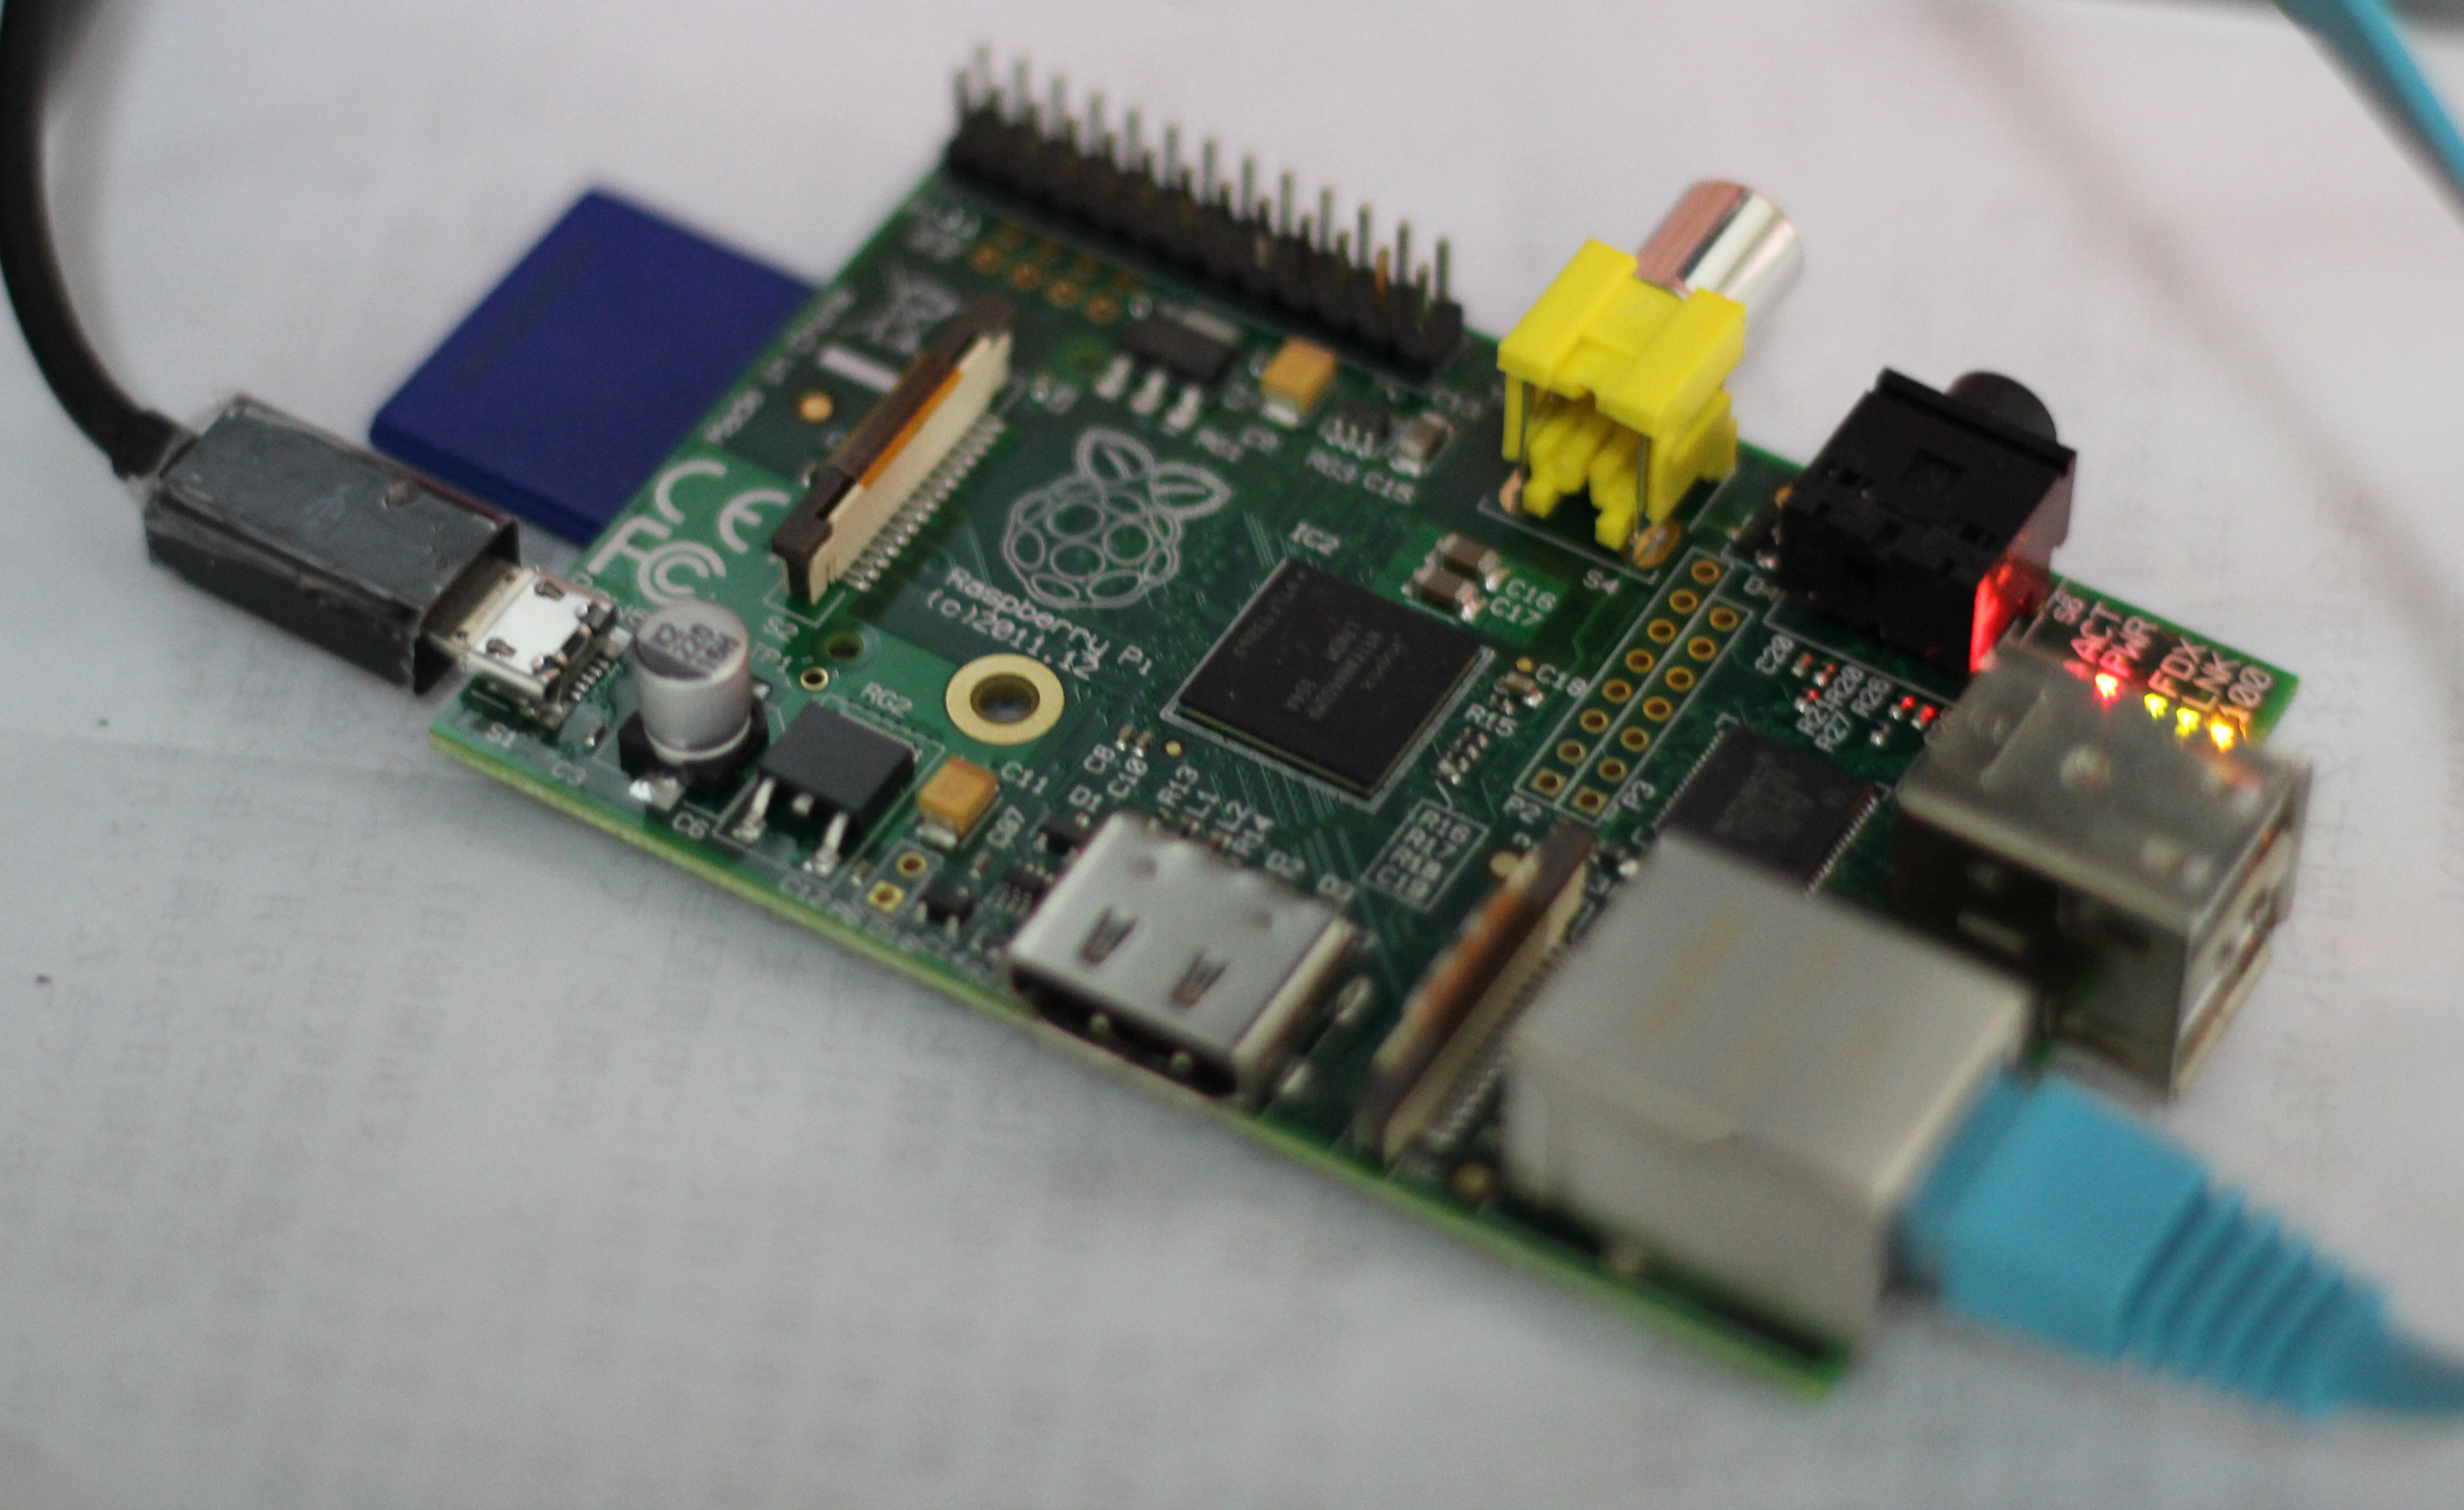
\includegraphics[width=1\hsize]{image201307/raspberrypi.jpg}
\end{frame}

\begin{frame}{raspbian}
 \begin{itemize}
  \item armel: armv4
  \item raspbian: armv6 (VFP2)
  \item armhf: armv7 (NEON)
 \end{itemize}
\end{frame}

\begin{frame}{raspbianのインストール}
\begin{itemize}
 \item SD-card にイメージを書き込んでそれから起動する
\end{itemize}
\end{frame}

\begin{frame}{サブマシンを使う時の便利技}
\begin{itemize}
 \item mosh: ssh 張りっぱなしな感じにできて、ノートパソコンサスペンドしてもリジューム
       したらまた繋げられる。
 \item avahi-daemon: DHCPの環境で面倒なことしなくても
       ホスト名指定でアクセスできるようになる。raspberrypi.local 
 \item sshfs: ssh でつながるホストのディレクトリを sshfsを使って透過的
       にマウントできる。NFSでユーザIDを調整したりSMBの設定を頑張ってし
       たりしていたのは過去のことに。
\end{itemize}
\end{frame}


\begin{frame}[containsverbatim]{小技:sshfs}
\begin{commandline}
 sshfs corei7.local:path/to/work ./mnt/
\end{commandline}
\end{frame}

\begin{frame}{raspbianのセンサー}
\begin{itemize}
 \item CPU温度センサーを使ってみた
\end{itemize}
  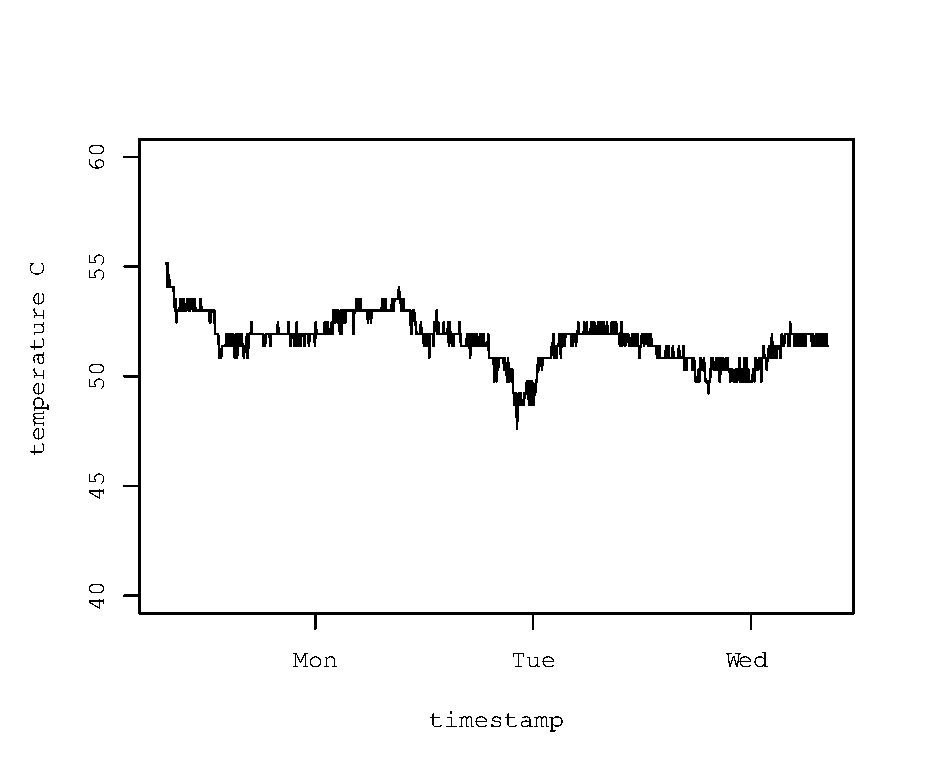
\includegraphics[width=0.8\hsize]{image201307/temperature.eps}
\end{frame}

\begin{frame}[containsverbatim]{sqlite + R}
時系列データを sqlite で保存
\begin{commandline}
create table temperature(
  timestamp TEXT default current_timestamp,
  temperature INTEGER);
\end{commandline}

定期的にシェルスクリプトで温度を書き込み
\begin{commandline}
while sleep 5m; do
    temp=$(cat /sys/class/thermal/thermal_zone0/temp)
    echo "insert into temperature(temperature) " \
 "values($temp);" | \
	sqlite3 sensor.db 
done 
\end{commandline}
\end{frame}

\begin{frame}[containsverbatim]{R でグラフ作成}
タイムゾーンUTCのPOSIXct 形式の文字列として解釈されるのでそれで処理して
 グラフ作成

\begin{commandline}
library("RSQLite")
drv <- dbDriver("SQLite", max.con=1)
conn <- dbConnect(drv, dbname='sensor.db')
r <- dbGetQuery(conn, 'SELECT * from temperature')
r$posix <- as.POSIXct(r$timestamp, tz='UTC')
plot((temperature / 1000) ~ posix, r,
     xlab='timestamp',
     ylab='temperature C',
     ylim=c(40,60), type='l')
\end{commandline}
\end{frame}

\begin{frame}{僕のraspberry piの今後}
多分こんなことします。
\begin{itemize}
 \item 1000円くらいで手に入る WebCamつけて監視システム
 \item 温度計つけて温度測定
\end{itemize}
\end{frame}

\section{今後のイベント}
\emtext{今後のイベント}
\begin{frame}{今後のイベント}
\begin{itemize}
 \item 2013年8月 Debian勉強会
\end{itemize}
\end{frame}

\section{今日の宴会場所}
\emtext{今日の宴会場所}
\begin{frame}{今日の宴会場所}
未定
\end{frame}

\end{document}

;;; Local Variables: ***
;;; outline-regexp: "\\([ 	]*\\\\\\(documentstyle\\|documentclass\\|emtext\\|section\\|begin{frame}\\)\\*?[ 	]*[[{]\\|[]+\\)" ***
;;; End: ***
